\section{\content{電腦中的漢字}{电脑中的汉字}}\label{section:chinese characters on computers}
\content{進入現代以後,電腦成為了人們讀寫漢字的新媒介。如今資訊科技高度發達,許多人使用電腦來讀寫的時間已經遠遠超過了使用紙筆。媒介的改變當然會帶來讀寫方式的改變,於是人們設計數位字型以供顯示漢字,設計輸入法以供鍵入漢字。}{进入现代以后,电脑成为了人们读写汉字的新媒介。如今信息技术高度发达,许多人使用电脑来读写的时间已经远远超过了使用纸笔。媒介的改变当然会带来读写方式的改变,于是人们设计数码字型以供显示汉字,设计输入法以供键入汉字。}\par
\content{在本節,筆者將簡要介紹一些電腦漢字相關的知識。如果你對「亂碼」的來歷感到好奇,對中文輸入法的選擇有些困惑,或者是想了解印刷體與手寫體的區別,那就一定不要錯過本節的內容。}{在本节,笔者将简要介绍一些电脑汉字相关的知识。如果你对“乱码”的来历感到好奇,对中文输入法的选择有些困惑,或是是想了解印刷体与手写体的区别,那就一定不要错过本节的内容。}\par
\subsection{\content{中文輸入法}{中文输入法}}
\content{我們一般所說的「輸入法」可以分解成兩個層次的概念:\textbf{輸入法方案}與\textbf{輸入法程式}。很多人在比較輸入法時,經常把方案之間的比較與程式之間的比較相混淆,從而引起很多不必要的爭執。筆者認為自己有義務對這些概念加以解釋。}{我们一般所说的“输入法”可以分解成两个层次的概念:\textbf{输入法方案}与\textbf{输入法程序}。很多人在比较输入法时,经常把方案之间的比较与程式之间的比较相混淆,从而引起很多不必要的争执。笔者认为自己有义务对这些概念加以解释。}\par
\subsubsection{\content{輪入法方案}{输入法方案}}
\content{輸入法方案關乎於每個字的編碼。在倉頡碼中「輸」的編碼是\charcode{十十人一弓},對應到鍵盤上就是\charcode{jjomn};在漢語全拼中的編碼則是\charcode{shu},對應鍵盤上的\charcode{shu}。}{输入法方案关乎于每个字的编码。在仓颉码中“输”的编码是\charcode{大手人一弓},对应到键盘上就是\charcode{kqomn};在汉语全拼中的编码则是\charcode{shu},对应键盘上的\charcode{shu}。}\par
\content{一種最死板的輸入法方案是,直接把所有漢字亂序編碼。我們只要強記這些編碼,就可以在鍵盤上打出任何一個想要的字。Unicode輸入法便是如此,我們只需敲下「輸」的編碼\charcode{8f38}就可以得到這個字。}{一种最死板的输入方案是,直接把所有汉字乱序编码。我们只要强记这些编码,就可以在键盘上打出任何一个想要的字。Unicode便入法便是如此,我们只需敲下“输”的编码\charcode{8f93}就可以得到这个字。}\par
\content{這類編碼的缺陷顯而易見:各個漢字與其編碼之間沒有任何邏輯關聯。為了正常使用,人們必須強行記住每個字的編碼,而這樣巨大的記憶量將使人望而卻步。所以人們當然更傾向於把漢字與其編碼關聯起來,用「推導」代替不必要的「記憶」。這種邏輯關聯的本質就是直接分析一個字的音、形、義,由此推算出編碼。分析字義並不可行,所以主流的中文輸入法要麼是基於字音的\textbf{音碼輸入法},要麼是基於字形的\textbf{形碼輸入法}。}{这类编码的缺陷显而易见:各个汉字与其编码之间没有任何逻辑关联。为了正常使用,人们必须强行记住每个字的编码,而这样巨大的记忆量将使人望而却步。所以人们当然更倾向于反汉字与其编码关联起来,用“推导”代替不必要的“记忆”。这种逻辑关联的本质就是直接分析一个字的音、形、义,由此推算出编码。分析字义并不可行,所以主流的中文输入法要么是基于字音的\textbf{音码输入法},要么是基于字形的\textbf{形码输入法}。}\par
\content{音碼輸入法的拆字思路比較簡單:根據漢語拼音、注音符號或粵語拼音等,把一個字的讀音轉換成編碼。「輸」的粵語拼音是\boxpinyin{syu},對應到粵拼方案上就是\charcode{syu};拼音是\boxpinyin{shu},對應到自然碼雙拼方案上就是\charcode{uu}\footnote{在自然碼雙拼中,聲母\boxpinyin{sh}對應到\charcode{u}鍵。此方案還提供了字形輔助碼,但那不是必需部分。};注音是\boxzhuyin{ㄕㄨ},對應到大千式注音方案上就是\charcode{gj}。對於受過良好拼音/注音教育的人來說,字音輸入法的優點就是上手簡單,易學易用——無論你是否會寫,只要你知道它的讀音,你就知道它在拼音/注音中如何拆,然後你只需要在鍵盤上敲下對應的鍵\footnote{在台灣,許多電腦鍵盤不止印有英數字母,還印有注音符號甚至倉頡、大易字根,所以在鍵盤上就可以直接找到注音符號的位置。}就可以了。}{音码输入法的拆字思路比较简单:根据汉语拼音、注音符号或粵语拼音等,把一个字的读音转换成编码。“输”的粵语拼音是\boxpinyin{syu},对应到粵拼方案上就是\charcode{syu};拼音是\boxpinyin{shu},对应到自然码双拼方案上就是\charcode{uu}\footnote{在自然码双拼中,声母\boxpinyin{sh}对应到\charcode{u}键。此方案还提供了字形辅助码,但那不是必需部分。};注音是“ㄕㄨ”,对应到大千式注音方案上就是\charcode{gj}。对于受过良好拼音/注音教育的人来说,字音输入法的优点就是上手简单,易学易用——无论你是否会写,只要你知道它的读音,你就知道它在拼音/注音中如何拆,然后你只需要在键盘上敲下对应的键\footnote{在台湾,许多电脑键盘不止印有英数字母,还印有注音符号甚至仓颉、大易字根,所以在键盘上就可以直接找到注音符号的位置。}就可以了。}\par
\begin{wrapfigure}{O}{.38\textwidth}
	\centering
	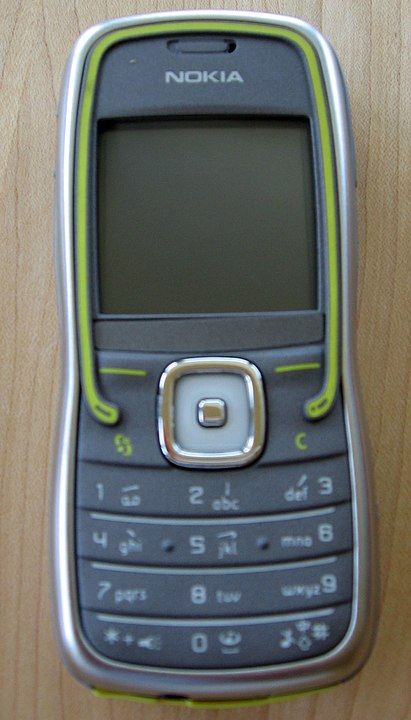
\includegraphics[width=.38\textwidth]{Nokia_5500.jpg}
	\caption{\content{一款諾基亞傳統型手機}{一款諾基亞傳統型手機}}
	\label{figure:一款諾基亞傳統型手機}
	\footnotesize{\color{darkgray}\content{鍵盤1-5對應有筆順鍵}{键盘1-5对应有笔顺键}}
\end{wrapfigure}
\content{音碼輸入法往往都基於既有的拼音/注音方案,在拆字思路上大同小異;但形碼輸入法就五花八門了。最細碎的筆畫輸入法把每個字的筆畫都拆開來,分成「橫竪撇點折」五類,每一筆都是一碼,那麼「輸」字要敲上足足16碼。因為編碼過長,輸入效率很低,所以幾乎沒有人再使用了,只在傳統型手機的九鍵鍵盤中還有保留(\cref*{figure:一款諾基亞傳統型手機})。}{音码输入法往往都基于既有的拼音/注音方案,在拆字思路上大同小异;但形码输入法就五花八门了。最细碎的笔画输入法把每个字的笔画都拆开来,分成“横竖撇点折”五类,每一笔者是一码,那么“输”字要敲上足足13码。因为编码过长,输入效率很低,所以几乎没有人再使用了,只在传统型手机的九键键盘中还有保留(\cref*{figure:一款諾基亞傳統型手機})。}\par
\content{很多字的成分非常複雜,一筆一畫寫出來不現實,所以我們需要限制每個字的編碼長度,只取其中的若干成分,作為\textbf{字根}。一個字的編碼將根據它的字根及結構來確定。四角號碼便是如此。它規定一個字必須編四碼\footnote{這里不考慮附角。如果考慮附角的話,應是五碼。},在編碼時分別看這個字左上角、右上角、左下角、右下角的字根形狀,再把字根轉換為對應的數字。還以「輸」字為例,它的左上角和左下角是連起來的一個「插」畫,所以左上角取\charcode{5},左下角用\charcode{0}代替;右上角的「人」是「八」畫,取\charcode{8};右下角的「亅」是「垂」畫,取\charcode{2}。所以「輸」字的四角號碼為\charcode{5802}。}{很多字的成分非常复杂,一笔一画写出来不现实,所以我们需要限制每个字的编码长度,只取其中的若干成分,作为\textbf{字根}。一个字的编码将根据它的字根及结构来确定。四角号码便是如此。它规定一个字必须编四码\footnote{这里不考虑附角。如果考虑附角的话,应是五码。},在编码时分别看这个字左上角、右上角、左下角、右下角的字根形状,再把字根转换为对应的数字。还以“输”字为例,这个字左上角的“𠂇”是“叉”画,取\charcode{4};右上角的“人”是“八”画,取\charcode{8};左下角的“𰀁”是“插”画,取\charcode{5};右下角的“亅”是“垂”画,取\charcode{2}。所以“输”字的四角号码为\charcode{4852}。}\par
\content{四角號碼發明於20世紀初。當時四角號碼並非用於打字,而是用於「檢字」\footnote{最典型的檢字就是根據字形查字典。很多人只會用部首檢字法,即:先根據部首的筆畫數量找到部首所在頁,再根據剩餘的筆畫數量從同部首的字中找到目標字。這種檢字方法容易學,但效率偏低,因為既要確定部首,又要數出筆畫數量,還需要在很多字中找到目標字。用四角號碼來檢字就方便很多。}。後來有人把四角號碼加以改良,製成縱橫輸入法。縱橫碼的思路也是根據漢字四角的成分來取碼。}{四角号码发明于20世世纪初。当时的四角号码并非用于打字,而是用于“检字”\footnote{最典型的检字就是根据字形查字典。很多人只会用部首检字法,即:先根据部首的笔画数量找到部首所在页,再根据剩余的笔画数量从同部首的字中找到目标字。这种检字方法容易学,但效率偏低,因为既要确这部首,又要数出笔画数量,还需要在很多字中找到目标字。用四角号码来检字就方便很多。}。后来有人把四角号码加以改良,制成纵横输入法。纵横码的思路也是根据汉字四角的成分来取码。}\par
\content{筆順、四角和縱橫所需的編碼鍵較少,所以在九鍵鍵盤或電腦小鍵盤上仍有用武之地;但在大鍵盤上,我們完全可以把字根分得更細緻。大易輸入法和行列40輸入法使用了40個鍵;行列30輸入法使用了30個鍵;鄭碼、徐碼、嘸蝦米使用了26個鍵;倉頡輸入法\footnote{不含六代倉頡輸入法(或曰「蒼頡輸入法」)。}、五筆字型輸入法使用了25個鍵\footnote{倉頡的\charcode{重}和五筆的\charcode{z}都不是必需的,不計入。}。}{笔顺、四角和纵横所需的编码键较少,所在在九键键盘或电脑小键盘上仍有用武之地;但在大键盘上,我们完全可以把字根分得更细致。大易输入法和行列40输入法使用了40个键;行列30输入法使用了30个键;郑码、呒吓米输入法使和了26个键;仓颉输入法\footnote{不含六代仓颉输入法(或曰“苍颉输入法”)。}、五笔字型输入法使用了25个键\footnote{仓颉的\charcode{重}和五笔的\charcode{z}都不是必需的,不计入。}。}\par
\content{不同的形碼輸入法可能採用完全不同的字根體系、拆字方式和編碼方式。但無論如何,只要給定一套規則,我們就可以對任何一個字進行編碼。這就是「輸入法方案」所關注的問題。}{不同的形码输入法可能采用完全不同的字根体系,拆字方式和编码方式。但无论如何,只要给定一套规则,我们就可以对任何一个字进行编码。这就是“输入法方案”所关注的问题。}\par
\subsubsection{\content{輸入法程式}{输入法程序}}
\content{筆者對形碼輸入法了解較多,常聽到有人比較形碼輸入法時給出這樣的說法:}{笔者对形码输入法了解较多,常听到有人比较形码输入法时给出这样的说法:}
\begin{itemize}
	\item \content{甲輸入法沒有容錯碼,有些字因為某些原因有多種拆碼方式,但人們只能按其中一種編碼來鍵入,換另一種合理的編碼卻打不出想要的字;乙輸入法卻有容錯碼。所以乙輸入法更好。}{甲输入法没有容错码,有些字因为某些原因有多种拆码方式,但人们只能按其中一种编码来键入,换另一种合理的编码却打不出想要的字;乙输入法却有容错码。所以乙输入法更好。}
	\item \content{甲輸入法只支援打簡體字,不支援打繁體字(或者正相反);乙輸入法既能打繁體字,又能打簡體字,還能打日本漢字、假名、諺文等。所以乙輸入法更好。}{甲输入法只支持打简体字,不支持打繁体字(或者正相反);乙输入法既能打繁体字,又能打简体字,还能打日本汉字、假名、谚文等。所以乙输入法更好。}
	\item \content{甲輸入法只能打些常用字,遇到生僻字就打不出來了;乙輸入法卻能打很多生僻字。所以乙輸入法更好。}{甲输入法只能打些常用字,遇到生僻字就打不出来了;乙输入法却能打很多生僻字。所以乙输入法更好。}
	\item ……
\end{itemize}
\content{這類說法有一個共性:它們本應是輸入法程式層面的比較,而不是輸入法方案層面的比較。然而人們常常把這些程式層面的問題延伸到方案上去,變成了「五筆打不了繁體字,來學倉頡」或者「倉頡不支援異體字,來學某某」云云,這是一種不自知的偷換概念。}{这类说法有一个共性:它们本应是输入法程式层面的比较,而不是输入法方案层面的比较。然而人们常常把这些程式层面的问题延伸到方案上去,变成了“五笔打不了繁体字,来学仓颉”或者“仓颉不支持异体字,来学某某”云云,这是一种不自知的偷换概念。}\par
\begin{wrapfigure}{O}{.3\textwidth}
	\centering
	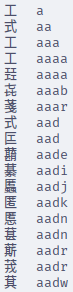
\includegraphics[width=.15\textwidth]{五筆碼表部分.png}
	\caption{\content{一份YAML格式的五筆碼表(部分)}{一份YAML格式的五笔码表(部分)}}
	\label{figure:一份YAML格式的五筆碼表}
\end{wrapfigure}
\content{電腦不會自動地根據輸入法方案所述的規則,對每個字進行編碼;這項工作必須由人來完成。輸入法程式的設計者需要按照輸入法方案的規則,把每個字的編碼確定下來,編成一張\textbf{碼表}。}{电脑不会自动地根据输入法方案所述的规则,对每个字进行编码;这项工作必须由人来完成。输入法程序的设计者需要按照输入法方案的规则,把每个字的编码确定下来,编成一张\textbf{码表}。}\par
\content{有了碼表之後,電腦才能根據你輸入的編碼,找到這個編碼對應的字——也就是你想要的字。以\cref*{figure:一份YAML格式的五筆碼表}為例,輸入五筆編碼\charcode{aadn}能得到「慝葚」兩個項,我們可以選字輸入。但是如果碼表中沒有「慝」呢?我們用\charcode{aadn}自然打不出「慝」字;候選項中只有「葚」這一個字。同樣的道理,\textbf{如果一個碼表中只有簡體字,我們就打不出繁體字;如果一個碼表中只有常用字,我們就打不出生僻字。}有人說「五筆輸入法打不出繁體字」,那是因為他所用的輸入法「程式」所帶碼表中沒有繁體字,並不是五筆輸入法這個「方案」本身不支援繁體字(實際上五筆方案是支援繁體字的,它有繁體字字根)。}{有了码表之后,电脑才能根据你输入的编码,找到这个编码对应的字——也就是你想要的字。以\cref*{figure:一份YAML格式的五筆碼表}为例,输入五笔编码\charcode{aadn}能得到“慝葚”两个项,我们可以选字输入。但是如果码表中没有“慝”呢?我们用\charcode{aadn}自然打不出“慝”字;候选项中只有“葚”这一个字。同样的道理,\textbf{如果一个码表中只有简体字,我们就打不出繁体字;如果一个码表中只有常用字,我们就打不出生僻字。}有人说“五笔输入法打不出繁体字”,那是因为他所用的输入法“程序”所带码表中没有繁体字,并不是五笔输入法这个“方案”本身不支持繁体字(实际上五笔方案是支持繁体字的,它有繁体字字根)。}\par
\content{容錯碼的處理也屬於程式方面的問題。就以「黃」字來說,它的港標寫法和台標寫法有著細微的不同:港標寫法是「{\hk 黃}」,中間是「由」字形;台標寫法則是「黃」,中間是「田」字形。如果某套倉頡輸入法碼表只考慮了港標字形而把此字編碼成\charcode{廿一中金}的話,台標用戶就會感到困惑:明明按「黃」字形拆成\charcode{廿一田金},卻怎麼也找不到這個字。一款做得細緻的輸入法程式會充分考慮到這種異寫造成的編碼不唯一問題,並採用有容錯碼的碼表;而有些輸入法程式就沒有考慮過這些問題。但是無論如何,\textbf{這個鍋應該交給輸入法程式來背,不該讓輸入法方案來背。}}{容错码的处理也属于程序方面的问题。就以“黄”字来说,它的港标写法与台标写法有着细微的不同:港标写法是“{\hk 黃}”,中间是“由”字形;台标写法则是“{\tw 黃}”,中间是“田”字形。如果某套仓颉输入法码表只考虑了港标字形而把此字编码成\charcode{廿一中金}的话,台标用户就会感到困惑:明明按“{\tw 黃}”字形拆成\charcode{廿一田金},却怎么也找不到这个字。一款做得细致的输入法程序会充分考虑到这种异写造成的编码不唯一问题,并采用有容错码的码表;而有些输入法程序就没有考虑过这些问题。但是无论如何,\textbf{这个锅应该交给输入法程序来背,不该让输入法方案来背。}}\par
\content{還有很多個性化的功能也是程式相關的,與方案無關。有些形碼輸入法支援形碼與拼音混輸,那是因為程式設計者把兩套碼表結合起來了;有些輸入法支援動態詞頻,那是因為輸入法程式有一套統計和計算方法;有些五筆輸入法允許四碼唯一自動上屏,以及第五碼頂字上屏,那是程式設計者為了提高輸入效率而做的功能優化;有些音碼輸入法支援模糊音\footnote{多數方言系統與普通話系統所含聲韻母不同,於是說慣了方言的人在學習普通話拼音時有可能分不清某些聲韻母,比如\bopin{ㄋ}{n}與\bopin{ㄌ}{l},\bopin{ㄣ}{en}與\bopin{ㄥ}{eng}等。很多拼音輸入法為了照顧這些群體,會設計出模糊音功能。這樣一來,敲\bopin{ㄕˋ}{\pinyin{shi4}}可以出「四」,敲\bopin{ㄙˊ}{\pinyin{si2}}也可以出「十」。},這也是程式設計者應該考慮的工作……凡此種種,不一而足。可是有些人在比較輸入法「方案」時卻有意或無意地把「程式」的優劣也拿來當作參考,那就不公平了!}{还有很多个性化的功能也是程序相关的,与方案无关。有些形码输入法支持形码与拼音混输,那是因为程序设计者把两套码表结合起来了;有些输入法支持动态词频,那是因为输入法程序有一套统计和计算方法;有些五笔输入法允许四码唯一自动上屏,以及第五码顶字上屏,那是程序设计者为了提高输入效率而做的功能优化;有些音码输入法支持模糊音\footnote{多数方言系统与普通话系统所含声韵母不同,于是说惯了方言的人在学习普通话拼音时有可能分不清某些声韵母,比如\bopin{ㄋ}{n}与\bopin{ㄌ}{l},\bopin{ㄣ}{en}与\bopin{ㄥ}{eng}等。很多拼音输入法为了照顾这些群体,会设计出模糊音功能。这样一来,敲\bopin{ㄕˋ}{\pinyin{shi4}}可以出“四”,敲\bopin{ㄙˊ}{\pinyin{si2}}也可以出“十”。},这也是程序设计者应该考虑的工作……凡此种种,不一而足。可是有些人在比较输入法“方案”时却有意无意地把“程序”的优劣也拿来当作参考,那就不公平了!}\par
\content{在輸入法領域,提出一套輸入法方案的人一般都要做一個輸入法程式並釋出,否則光有方案沒有程式,就是紙上談兵。其他人也可能根據這套方案,自行設計輸入法程式;甚至改良原有方案,做成更適合某些受眾的新方案,再做成輸入法程式。Rime輪入引擎更是提供了高度個性化的選擇,使用戶能夠自定義輸入法的功能、碼表——通俗點說,用戶可以利用Rime自己設計輸入法程式,不用擔心市面上的輸入法沒有自己想要的功能。所以時至今日,我們不應該再拿「輸入法程式」層面的指標去作比較了,因為「你有什麼功能,我也可以有;哪怕現在沒有,我也可以做給你看」。但作為輸入法之核心的「方案」,才能真正決定一個字「應該怎麼拆、應該怎麼編碼」,這才是我們比較輸入法時真正應該思考的部分。}{在输入法领域,提出一套输入法方案的人一般都要做一个输入法程序并发布,否则光有方案没有程序,就是纸上谈兵。其他人也可能根据这套方案,自行设计输入法程序;甚至改良原有方案,做成更适合某些受众的新方案,再做成输入法程序。Rime输入引擎更是提供了高度个性化的选择,使用户能够自定义输入法的功能、码表——通俗点说,用户可以利用Rime自己设计输入法程序,不用担心市面上的输入法没有自己想要的功能。所以时至今日,我们不应该再拿“输入法程序”层面的指标去作比较了,因为“你有什么功能,我也可以有;哪怕现在没有,我也可以做给你看”。但作为输入法之核心的“方案”,才能真正决定一个字“应该怎么拆、应该怎么编码”,这才是我们比较输入法时真正应该思考的部分。}\par
\subsubsection{\content{音碼、形碼與音形碼}{音码、形码与音形码}}
\content{前面說過,主流輸入法基本分為音碼輸入法與形碼輸入法。當然也有二者結合的音形碼輸入法。}{前面说过,主流输入法基本分为音码输入法与形码输入法。当然也有二者结合的音形码输入法。}\par
\content{有些音形碼方案的設計初衷在於降低音碼方案的\textbf{重碼率}——漢字中的同音字太多,如果純用音碼的話,會有很多字編碼相同\footnote{筆者簡單統計了一下,自己所用的拼音碼表中有797個\bopin{ㄧ}{yi}音的字,351個\bopin{ㄕ}{shi}音的字和301個\bopin{ㄨ}{wu}音的字。保守估計,非生僻字至少佔到10\%,這就意味著同一編碼下可能有數十個常見字。},我們不得不翻好幾頁來選詞,這樣就極大影響了輸入效率。雙拼方案可以有效地減少編碼長度,把每一字固定在2碼長,但對降低重碼率沒有幫助。既然依賴字音不能降低重碼,那麼還是要從字形出發,把同音字從編碼上分開來。}{有些音形码方案的设计初衷在于降低音码方案的\textbf{重码率}——汉字中的同音字太多,如果纯用音码的话,会有很多字编码相同\footnote{笔者简单统计了一下,自己所用的拼音码表中有797个\bopin{ㄧ}{yi}音的字,351个\bopin{ㄕ}{shi}音的字和301个\bopin{ㄨ}{wu}音的字。保守估计,非生僻字至少占到10\%,这就意味着同一编码下可能有数十个常见字。},我们不得不翻好几页来选词,这样就极大影响了输入效率。双拼方案可以有效地减少编码长度,把每一字固定在2码长,但对降低重码率没有帮助。既然依赖字音不能降低重码,那么还是要从字形出发,把同音字从编码上分开来。}\par
\content{小鶴音形就是這樣一種音形碼方案。它規定每個字最多編四碼,前兩碼為雙拼碼(音碼),後兩碼為形碼。比如「衣」和「佚」字,它們的雙拼都是\charcode{yi};但若加上後兩碼的形碼,就分別變成\charcode{yiwy}和\charcode{yiru},這樣就減少了重碼。自然碼雙拼方案也採用了形碼作為輔碼。雖然這些輸入方案都是音形碼,但用戶完全可以無視「形」的部分,純粹將其當成音碼輸入法來用。}{小鹤音形就是这样一种音形码方案。它规定每个字最多编四码,前两码为双拼码(音码),后两码为形码。比如“衣”和“佚”字,它们的双拼都是\charcode{yi};但若加上后两码的形码,就分别变成\charcode{yiwy}和\charcode{yiru},这样就减少了重码。自然码双拼方案也采用了形码作为辅码。虽然这些输入方案都是音形码,但用户完全可以无视“形”的部分,纯粹将其当成音码输入法来用。}\par
\content{有些音形碼輸入法則必須嚴格包含音形兩部分,二筆音形輸入法便是如此。它規定,一個字最多編四碼,第一碼取拼音首字母,後三碼按筆順取筆畫\footnote{就形碼的處理來說,二筆音形要比原始的筆畫輸入法高明些;但它的缺陷還是有很多,後文再談。感興趣的讀者可以自行查詢二筆輸入法的相關資料。}。以「輸」字為例,它的拼音是\boxpinyin{\pinyin{shu1}},所以第一碼取\charcode{s}。後三碼根據字形及結構取\charcode{jrk},這裡就不詳細解釋了。}{有些音形码输入法则必须严格包含音形两部分,二笔音形输入法便是如此。它规定,一个字最多编四码,第一码取拼音首字母,后三码按笔顺取笔画\footnote{就形码的处理来说,二笔音形要比原始的笔画输入法高明些;但它的缺陷还是有很多,后文再谈。感兴趣的读者可以自行查询二笔输入法的相关资料。}。以“输”字为例,它的拼音是\boxpinyin{\pinyin{shu1}},所以第一码取\charcode{s}。后三码根据字形及结构取\charcode{;rk},这里就不详细解释了。}\par
\content{不少人對嚴格的音形碼持批評態度,因為用戶在鍵入時必須要既知其音,又知其形。「齷齪」比較難寫,許多人不記得字形,但用音碼輸入法就可以很方便地打出來;「轡」「蠹」二字比較生僻,許多人不知道讀音,但用形碼輸入法也可以打出來\footnote{這種情況一般出現於需要依字形檢字的場合,或者抄錄內容的場合。總之,使用者知道或能看到字形,但不知道讀音。若是音、形全都不知道,那就根本沒辦法,不在討論之列。}。然而若是用了音形碼呢?以上兩類字全都不會打。所以僅就這個方面來說,音形碼的缺陷比單純的音碼、形碼都要大。}{不少人对严格的音形码持批评态度,因为用户在键入时必须要既知其音,又知其形。“龌龊”二字比较难写,许多人不记得字形,但用音码输入法就可以很方便地打出来;“辔”“蠹”二字比较生僻,许多人不知道读音,但用形码输入法也可以打出来\footnote{这种情况一般出现于需要依字形检字的场合,或者抄录内容的场合。总之,使用者知道或能看到字形,但不知道读音。若是音、形全都不知道,那就根本没办法,不在讨论之列。}。然而若是用了音形码呢?以上两类字全都不会打。所以仅就这个方面来说,音形码的缺陷比单纯的音码、形码都要大。}\par
\content{而自然碼、小鶴這些雙拼方案就比較靈活。它們雖然是音形碼方案,但我們完全可以把它當作音碼方案來用,所以不知道字形也沒有什麼大礙(有不少用戶壓根不學輔碼部分,也一樣能用好雙拼)。}{而自然码、小鹤这些双拼方案就比较灵活。它们虽然是音形码方案,但我们完全可以把它当作音码方案来用,所以不知道字形也没有什么大碍(有不少用户压根不学辅码部分,也一样能用好双拼)。}\par
\content{音碼的重碼率問題是由音碼方案本身所決定的,無法避免。音形碼方案能在一定程度上降低重碼率,但是,一方面,它要求用戶兼知音形才能打出一個字來;另一方面,很多音形碼方案只能降低單字重碼率,而無法降低詞組重碼率——例如,雙拼方案在輸入詞組時,只取每字的音碼,不取輔碼。恐怕只有純形碼方案能做到比較低的重碼率了。}{音码的重码率问题是由音码方案本身所决定的,无法避免。音形码方案能在一定程度上降低重码率,但是,一方面,它要求用户兼知音形才能打出一个字来;另一方面,很多音形码方案只能降低单字重码率,而无法降低词组重码率——例如,双拼方案在输入词组时,只取每字的音码,不取辅码。恐怕只有纯形码方案能做到比较低的重码率了。}\par
\content{在中文輸入法發展的早期,形碼曾因為低重碼、快速、適合盲打而受到許多人(尤其是專業人士)的青睞。後來音碼輸入法在「程式」層面做了諸多改進,比如智慧選字、動態詞頻、雲端詞庫、整句輸入、長句聯想等功能,使得輸入法程式越來越易用。這樣一來,雖然重碼率沒有下降,但「概率最高的選項」往往能排在最靠前的位置,於是用戶就可以少受翻頁選詞之苦了。}{在中文输入法发展的早期,形码曾因为低重码、快速、适合盲打而受到许多人(尤其是专业人士)的表睐。后来音码输入法在“程序”层面做了诸多改进,比如智能选字、动态词频、云端词库、整句输入、长句联想等功能,使得输tyif程序越来越易用。这样一来,虽然重码率没有下降,但“概率最高的选项”往往能排在最靠前的位置,于是用㧀不可以少受翻页选词之苦了。}\par
\content{對於音碼輸入法\footnote{尤指有智慧功能的音碼輸入法。現在市面上流行的大多數輸入法程式都或多或少配備這些功能了。}來說,\textbf{以詞為單位,甚至以短語/整句為單位來輸入,能夠有效提高輸入法的效率}。這點很好理解:如果別人用語音說了單獨一個字,你幾乎猜不到他說的到底是哪個字,因為同音字太多了;如果他說了一個詞,你大概能猜到幾個可能性,但未必能完全確定;而如果他說了一個短語或者一句話,那你幾乎就可以猜到每個字都是什麼了。這是因為,上下文為我們判斷文字提供了資訊量。對於智慧型輸入法來說,也是如此。}{对于音码输入法\footnote{尤指有智能功能的音码输入法。现在市面上流行的大多数输入法程序都或多或少配备这些功能了。}来说,\textbf{以词为单位,甚至以短语/整句为单位来输入,能够有效提高输入法的效率}。这点很好理解:如果别人用语音说了单独一个字,你几乎猜不到他说的到底是哪个字,因为同音字太多了;如果他说了一个词,你大概能猜到几个可能性,但未必能完全确定;而如果他说了一个短语或者一句话,那你几乎就可以猜到每个字都是什么了。这是因为,上下文为我们判断文字提供了信息量。对于智能输入法来说,也是如此。}\par
\content{而形碼輸入法則相反,\textbf{以詞組為單位來輸入,未必能提高輸入法的效率}。不僅如此,動態詞頻等智慧功能還可能成為輸入法使用過程中的跘腳石。形碼方案基本上無法區分一段編碼有幾個字\footnote{對於音碼編碼來說就很容易。大部分漢字都是有聲母的,所以在處理編碼時,從聲母處斷開就可以解決九成以上的斷字問題。},於是對於一個四碼長的編碼來說,單字、二字詞、三字詞等都會出現在候選項中。本來,單字的重碼率並不高;但加上詞組之後,候選項就變多了,重碼率也就增加了。換句話說,用單字時重碼少到幾乎可以盲打,但用單字/詞組混合時重碼卻多到很難支援我們盲打了。動態詞頻也有類似的問題:如果某字時而在第一位,時而在第二位,那麼我們就不能依靠盲打的記憶慣性來敲出此字了。}{而形码输入法则相反,\textbf{以词组为单位来输入,未必能提高输入法的效率}。不仅如此,动态词频等智能功能还可能成为输入法使用过程中的跘脚石。形码方案基本上无法区分一段编码有几个字\footnote{对于音码编码来说就很容易。大部分汉字都是有声母的,所以在处理编码时,从声母处断开就可以解决九成以上的断字问题。},于是对于一个四码长的编码来说,单字、二字词、三字词等都会出现在候选项中。本来,单字的重码率并不高;但加上词组之后,候选项就变多了,重码率也就增加了。换句话说,用单字时重码少到几乎可以盲打,但用单字/词组混合时重码却多到很难支持我们盲打了。动态词频也有类似的问题:如果某字时而在第一位,时而在第二位,那么我们就不能依靠盲打的记忆惯性来敲出此字了。}\par
\content{然而輸入時用單字不用詞組,無疑會減慢打字的速度——這也是形碼輸入法面臨的一個尷尬之處。面對這些問題,大概每個用戶都會做出自己的選擇吧!}{然而输入时用单字不用词组,无疑会减慢打字的速度——这也是形码输入法面临的一个尴尬之处。面对这些问题,大概每个用户都会做出自己的选择吧!}\par
